\documentclass[10pt,letterpaper]{article}
\usepackage[margin=0.55in]{geometry}
\usepackage{amsmath,amssymb,booktabs,tabularx}
\usepackage[T1]{fontenc}
\usepackage{lmodern}
\usepackage{microtype}
\usepackage{graphicx}
\usepackage[hidelinks]{hyperref}
\hypersetup{pdftitle={A conditional loss-budget bound for slope growth}}
\setlength{\parindent}{0pt}
\setlength{\parskip}{3pt}
\setlength{\abovedisplayskip}{3pt}
\setlength{\belowdisplayskip}{3pt}
\setlength{\abovedisplayshortskip}{3pt}
\setlength{\belowdisplayshortskip}{3pt}
\setlength{\tabcolsep}{7pt}
\renewcommand{\arraystretch}{1.15}
\begin{document}
\fontsize{9.5}{10.6}\selectfont
{\large\bfseries A conditional loss-budget bound for slope growth\par}
\vspace{4pt}
Rather than accumulating a positive growth allowance at every update, we relate outward slope motion to the remaining decrease in training error. This gives a bound with no explicit dependence on the number of steps, provided a gradient-direction condition persists.

\textbf{Theorem (slope-growth budget).}
Consider joint GD, $\theta_{n+1}=\theta_n-\eta g_n$, with constant $\eta>0$, full gradient $g_n=\nabla L(\theta_n)$, and squared loss $L=\tfrac12\operatorname{mean}[(q_\theta-y)^2]$. Let $\gamma_n\in\mathbb R^W$ be the slope block, $g_{\gamma,n}$ its gradient, and $E_n=\sqrt{2L_n}$ the full training residual RMS. Index zero may denote any restart. Suppose that, for every $n<T$,
\begin{equation}
L_{n+1}\le L_n-\frac{\eta}{2}\|g_n\|^2,
\qquad
E_n[-\langle\gamma_n,g_{\gamma,n}\rangle]_+
\le K\|g_n\|^2,
\end{equation}
where $K\ge0$ is fixed and $[z]_+=\max(z,0)$. Then, for every $n\le T$,
\begin{equation}
\|\gamma_n\|^2
\le\|\gamma_0\|^2+4K(E_0-E_n)+2\eta(L_0-L_n).
\end{equation}
In particular, writing $\gamma_{\mathrm{RMS},n}=\|\gamma_n\|/\sqrt W$,
\begin{equation}
\boxed{
\gamma_{\mathrm{RMS},n}
\le\sqrt{\gamma_{\mathrm{RMS},0}^{\,2}+
\frac{4KE_0+\eta E_0^2}{W}}.
}
\end{equation}

\textbf{Proof.}
Write $A_n=\|\gamma_n\|^2$. For $E_n>0$, the exact slope update and (1) give
\[
A_{n+1}-A_n
=-2\eta\langle\gamma_n,g_{\gamma,n}\rangle
+\eta^2\|g_{\gamma,n}\|^2
\le\frac{2\eta K}{E_n}\|g_n\|^2+\eta^2\|g_n\|^2.
\]
Meanwhile, sufficient decrease implies
\[
E_n-E_{n+1}
=\frac{2(L_n-L_{n+1})}{E_n+E_{n+1}}
\ge\frac{\eta\|g_n\|^2}{2E_n}.
\]
Consequently,
\[
A_{n+1}-A_n
\le4K(E_n-E_{n+1})+2\eta(L_n-L_{n+1}).
\]
Summing proves (2); nonnegativity of $E_n,L_n$ proves (3). If $E_n=0$, squared loss has $g_n=0$ and GD remains stationary.\nobreak\hfill$\square$

The second condition in (1) preserves the signed aggregate slope motion. Its measurable diagnostic is
\[
k_n=\frac{E_n[-\langle\gamma_n,g_{\gamma,n}\rangle]_+}{\|g_n\|^2},
\]
with $k_n=0$ when $g_n=0$. Bounding $k_n$ limits how much slope energy can increase per unit reduction in residual. The proof uses GD and squared loss; it does not require a tanh expansion or a small initial parameter norm.

\textbf{Empirical evaluation.}
We audited saved full-batch, float64 tanh GD trajectories for 24 functions, width 196, learning rates $10^{-3}$ and $10^{-4}$, and 1,024 training points. Targets have unit training RMS. Three initialization settings use the same paired seed: PyTorch defaults, and the same draw with first-layer weights and biases multiplied by two or four, leaving the initial readout unchanged. This gives 48 runs per setting.

We set one common $K=1000.273$ to twice the largest $k_n$ observed on the default-initialization 20k--30k prefixes, then froze it. We checked the later checkpoints through 200k, spaced 500 updates apart, and tested the same threshold on both larger initializations without retuning. Each ceiling in (3) uses that run's slopes and residual at 30k. The separate sufficient step-size test passed for all 144 analyzed continuations.

\begin{center}
\small
\begin{tabularx}{\linewidth}{@{}l>{\centering\arraybackslash}Xrr@{}}
\toprule
Initialization & Condition passes at all checked states & Largest $k_n$ & \shortstack{Largest RMS ceiling\\(passing runs)}\\
\midrule
Default & 48/48 & 924.76 & 4.55\\
$2\times$ & 47/48 & 1389.41 & 4.66\\
$4\times$ & 48/48 & 848.55 & 5.07\\
\bottomrule
\end{tabularx}
\end{center}
The failed case is Airy with $2\times$ initialization and learning rate $10^{-3}$; no guarantee under the fixed threshold is assigned to that run. The passing ceilings lie below the QUILL construction reference, 18.375. This comparison concerns RMS scale, not the maximum individual slope or a necessary threshold for accurate approximation.

\textbf{Scope.}
The theorem requires (1) at every update. These exploratory, floating-point checkpoint checks establish neither between-checkpoint persistence nor indefinite validity; some later states were inspected while developing the diagnostic. In particular, $k_n$ can diverge even along a bounded trajectory approaching a positive residual floor, and several measured curves are still increasing at 200k. Thus (3) is a horizon-independent \emph{conditional} bound, with empirical support over the recorded window, not a proof of permanent confinement.

\clearpage
\begin{figure}[!ht]
\centering
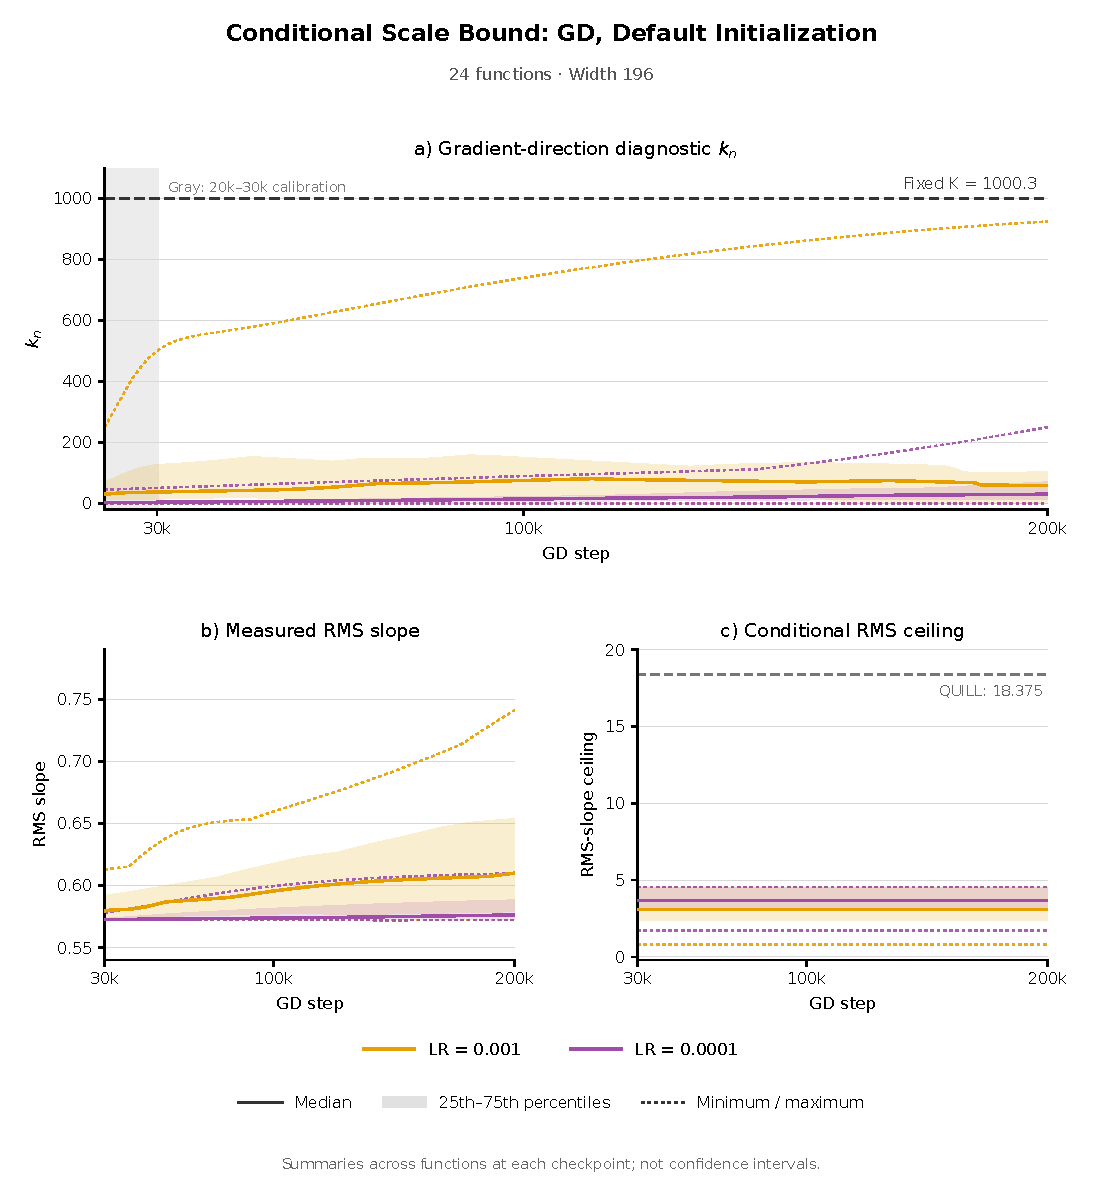
\includegraphics[width=\linewidth]{images/radial_loss_budget_distributions.pdf}
\caption{\small Distribution across the 24 functions, separately for each learning rate, under default initialization. Solid lines are medians, shaded bands span the 25th--75th percentiles, and dotted boundaries are the minima and maxima. Panel (a) shows the diagnostic $k_n$ and the fixed threshold calibrated over 20k--30k. Panel (b) shows measured RMS slopes. Panel (c) shows the constant conditional ceilings from (3), calculated at 30k, alongside the QUILL construction reference. These are across-function summaries from one paired seed, not confidence intervals. The ceilings require the theorem's premises at every update.}
\label{fig:k-distributions}
\end{figure}

\end{document}
